\documentclass[
	%a4paper, % Use A4 paper size
	letterpaper, % Use US letter paper size
]{jdf}

\addbibresource{references.bib}

\author{Alejandro Diaz}
\email{adiaz77@gatech.edu}
\title{Homework 1}

\begin{document}
%\lsstyle

\maketitle

\section{Question 1}
It is possible to represent the Star Wars problem as a semantic net. Each node of the net represents a state in the problem space. For the Star Wars problem, each node, at a minimum, should provide a way to store who is planet-side and where the ship's position (we do not have to store both sides because we can use one side to deduce the other so long as we know the total number of passengers in the problem). The operator between states will be the transition of the shuttle and its passenger choice. \textbf{\textit{Figure 1}} illustrates the semantic network created by abstracting the problem. 

\begin{figure}[h]
	\centering
	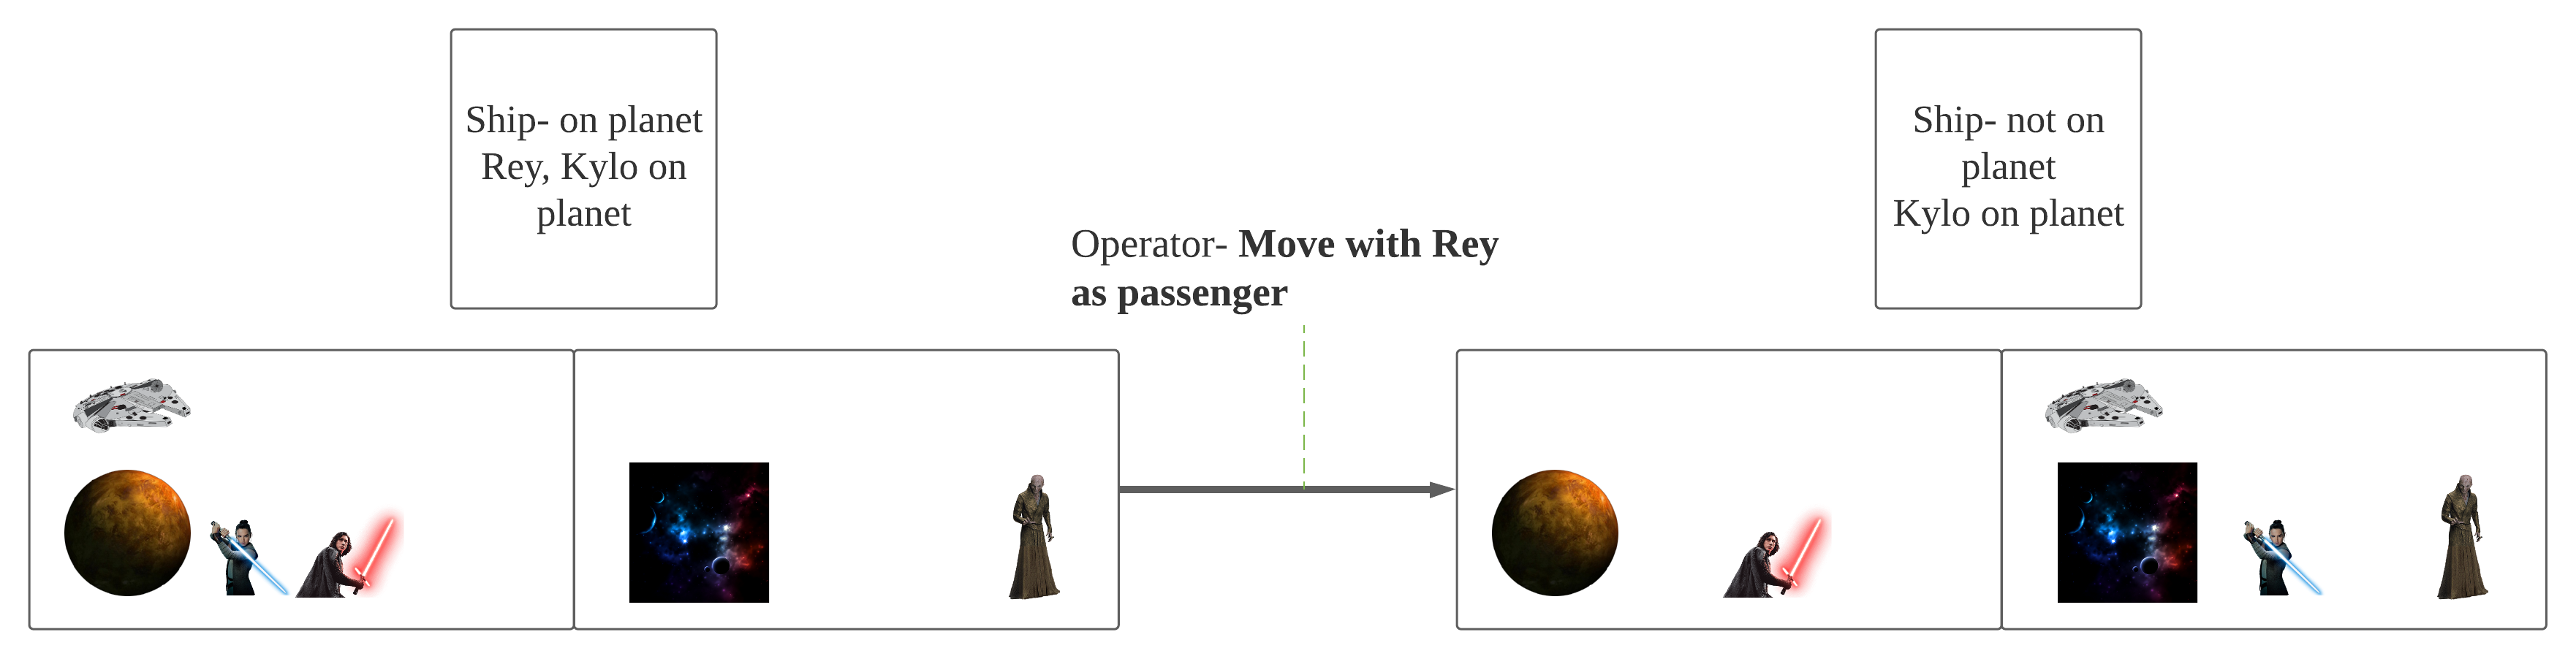
\includegraphics[height=11cm]{Figures/HW1 diagram - Page 2 (4).png}
	\caption{An example of a representation of the problem using a semantic net. Source: Star Wars used with Fair-Use, non-commercial  license (\cite{pngegg_contributor_star_nodate}et. all). Diagram by author.}
	\label{fig1:net}
\end{figure}

The generator should use the operator (move 1 or 0 passengers) to generate each possible state. The generator can generate $\textit{j} + 1$ cases, where $\textit{j}$ is the number of people on the same side as the ship. In turn, the tester should check each generated state for validity using the conditions listed.

\begin{itemize}
	\item State adheres to rules of the problem
	\item Checking if the state is a solution
	\item Checking to see if the state has been generated before along the path
	\item Merging any identical states on the same level to reduce branching
	\item Using breadth first search to navigate the net. Worst case time and space efficiency of $O(\textit{b}^d)$, where $\textit{b}$ is the branching factor and $\textit{d}$ is the depth (\cite{korf_artificial_1999})
\end{itemize}

\begin{figure}[hbtp]
	\centering
	
\includegraphics[width=\paperwidth,height=0.80\paperheight]{Figures/HW1 diagram - Page 1.png}
	\label{fig2:net}
	\caption{}
\end{figure}

\section{Question 2}
The General Data Protection Regulation (GDPR) outlines the principles by which companies must treat personal data. The regulation says that personally identifiable data must be consented for, processed fairly and transparently, collected with explicit consent, adequately (i.e., no blanket data-collection), accurately and limited to what is necessary (i.e., data minimization), handled, and stored to meet expectations outlined by the policy (\cite{european_parliament_general_2016})(\cite{davies_personalization_2018}). 

The regulation outlines how personal data may be used to personalize individual user experiences online. It makes the blanket data collection method illegal (Ch.2 Article V). Service providers can no longer collect personal data on implicit agreements; instead, GDPR requires explicit consent (Ch.2 Article VII). Data must now be opt-in and not opt-out. Services can no longer have a “take it or leave it” approach to their services. Any personal data collectors must offer users the ability to opt-out of personal data collection. Furthermore, GDPR outlines that any personal data that they store should be pseudonymization (Ch.4 Article XXVII). GDPR also allows users to choose to object to certain data processing and request that companies not process their data in such a way (Ch. 3 Article XXI).

Each of these personal data gathering policies has the potential to hinder AI and machine learning algorithms that offer user personalization. In cases where data must be anonymize or users otherwise withdraw consent to data collection or processing, the AI algorithm is working without data for its production model. In such cases, the agent will only be able to work with generic, non-personalized data such as geography, language, and otherwise aggregate data. The agent could use a matching algorithm to find similar personalized data profiles to apply to the anonymized user, but this goes against the spirit of the law. In short, data collectors (including for AI purposes) must ask for informed, categorical consent from users to collect relevant data. 

The night that the regulation went into effect, Google was sued for data collection concerns and lost the lawsuit (\cite{satariano_google_2019}). Google's products, such as their web search, have succeeded more so than any traditional advertisement because of their ability to build an advertising profile on their users.  

There were concerns that Google's personalized advertising would be hampered by the GDPR and the fallout of privacy court cases (\cite{barry_gdpr_2019}) Others argued that AI profiling could replace personal data with contextualization and solve Google's data problems (\cite{davies_personalization_2018}). Is there a world where these personalized advertising profiles can coexist with the GDPR?  

There is room for google to adapt. If Google provides transparency into what data is collected and for what purpose, users can agree to consent to allow Google to store a profile on them. Google should process their data transparently and inform users what the data is being used for and for how long. If Google can maintain personalization in their products but lose it in their advertisement, they will still survive. Their products will maintain large user bases that they can advertise too with or without personalization. AI and other personalizing tools are still possible in the EU. Google has other sources of data to draw from that does not violate personal user data. Google would be able to make highly personalized data best on aggregate trends and applying those trends to user groups. 

\section{References}
\printbibliography[heading=none]

\end{document}